\section{Heavy Higgs Interference Effects}
\label{sec:HHIntf}
% ---- ---- ---- ---- ---- ---- ---- ---- ---- ---- ---- ---- ---- ---- ---- ---- ---- ---- ---- ---- ---- ---- ----

With increasing Higgs mass, the interference effect becomes more and
more crucial between the signal $gg\to H \to WW$ and the continuum
background $gg \to WW$. As shown in Ref.~\cite{Campbell:2011cu}, the
effect on LO total cross sections is already over 30\% for $M_H\gtrsim
600$\,GeV. Moreover, it changes the $M_{WW}$ spectrum substantially, with
constructive behavior for $M_{WW}\lesssim M_H$ and destructive for
$M_{WW} \gtrsim M_H$. One usually can include the interference effects
by reweighting the signal's $M_{WW}$ distributions with $(1+R2)$,
where the ratio $R_2$ is defined as

\begin{equation}
R_{2} \equiv \frac{Intf}{S},
\label{R2}
\end{equation}

However, one needs then to validate the method by studying other
distributions than $M_{WW}$. In addition, one should include
conservative yet appropriate estimations on uncertainty of $R_2$.

In our study, we evaluate $R_2$ with LO $Intf$ and $S$ obtained from
the MCFM v6.3 (without any cuts applied). We then exploit the method
proposed in Ref.~\cite{Passarino:2012ri} to estimate the reweighting
uncertainty with 3 kinds of $R_2$ inspired by higher order QCD
corrections:

\begin{equation}
R_{2} = 1,\,\, \sqrt{K_{gg}}/K_{NNLO},\,\, {\rm and}\,\, 1/K_{NNLO},
\label{R2un}
\end{equation}

where the K factors $K_{gg}$ and $K_{NNLO}$ are read from the $H\to
ZZ$ numbers in Ref.~\cite{Passarino:2012ri}, as the ones for $H\to WW$
are not ready yet, and the K factors should not depend on final states
between $gg\to H\to WW$ and $ZZ$.

In Fig.~\ref{fig:MCFMHHIntfRew}, we show our reweighting results for
$gg\to H \to WW \to l\nu jj$ at the generator level, for
$M_H=700$\,GeV at the 8TeV LHC, with $P_{T,l}>30$\,GeV,
$P_{T,j}>30$\,GeV, MET$>30$\,GeV, and $|\eta_{l,j}|<2.4$. The
reweighting based on $M_{WW}$ spectrum turns out to decribe well the
other distributions. The uncertainty band on interference effect
reweighting, as mentioned above, is also provided for various
distributions.

%
\begin{figure}[htb]
    \subfigure[$M_{WW}$]{
      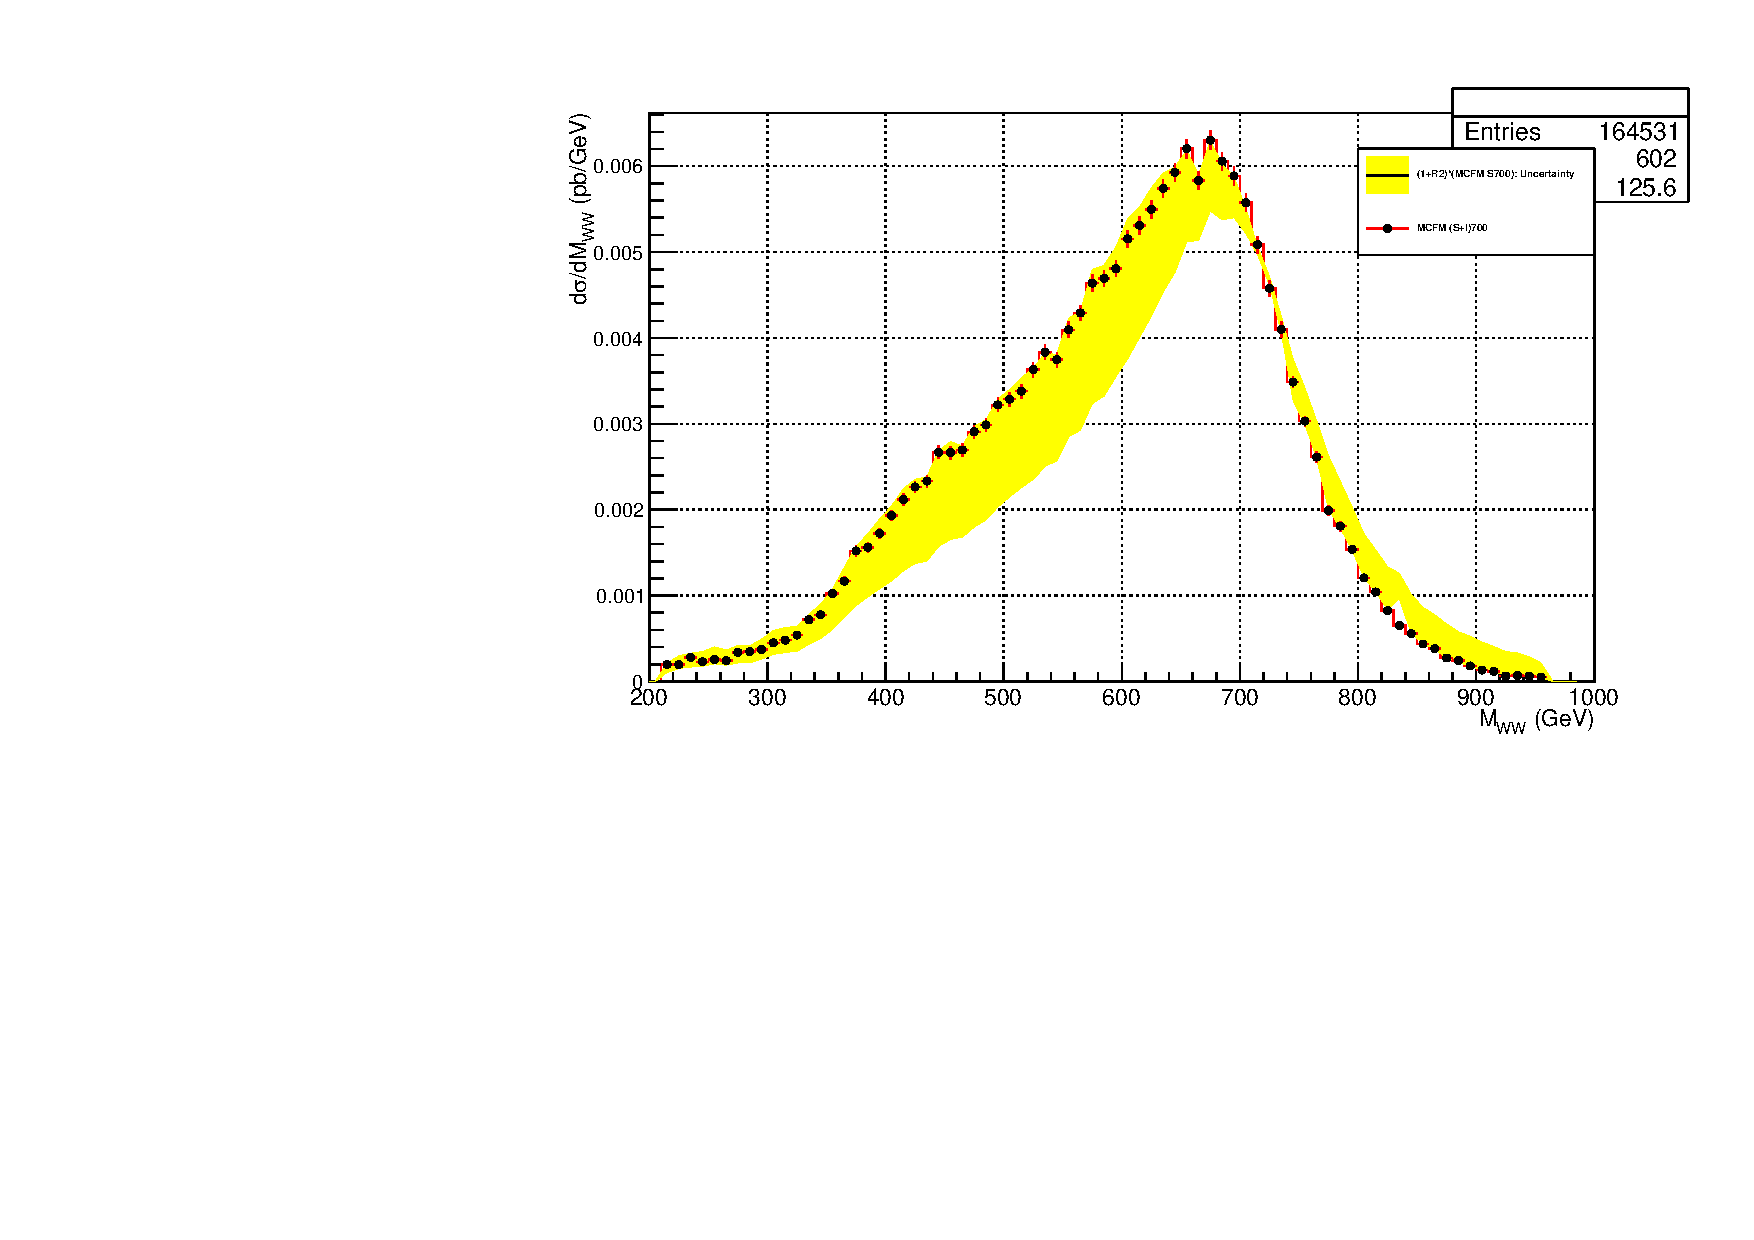
\includegraphics[width=0.42\textwidth]{plots/interference/mww.pdf}
    }
    \subfigure[$M_{l\nu}$]{
      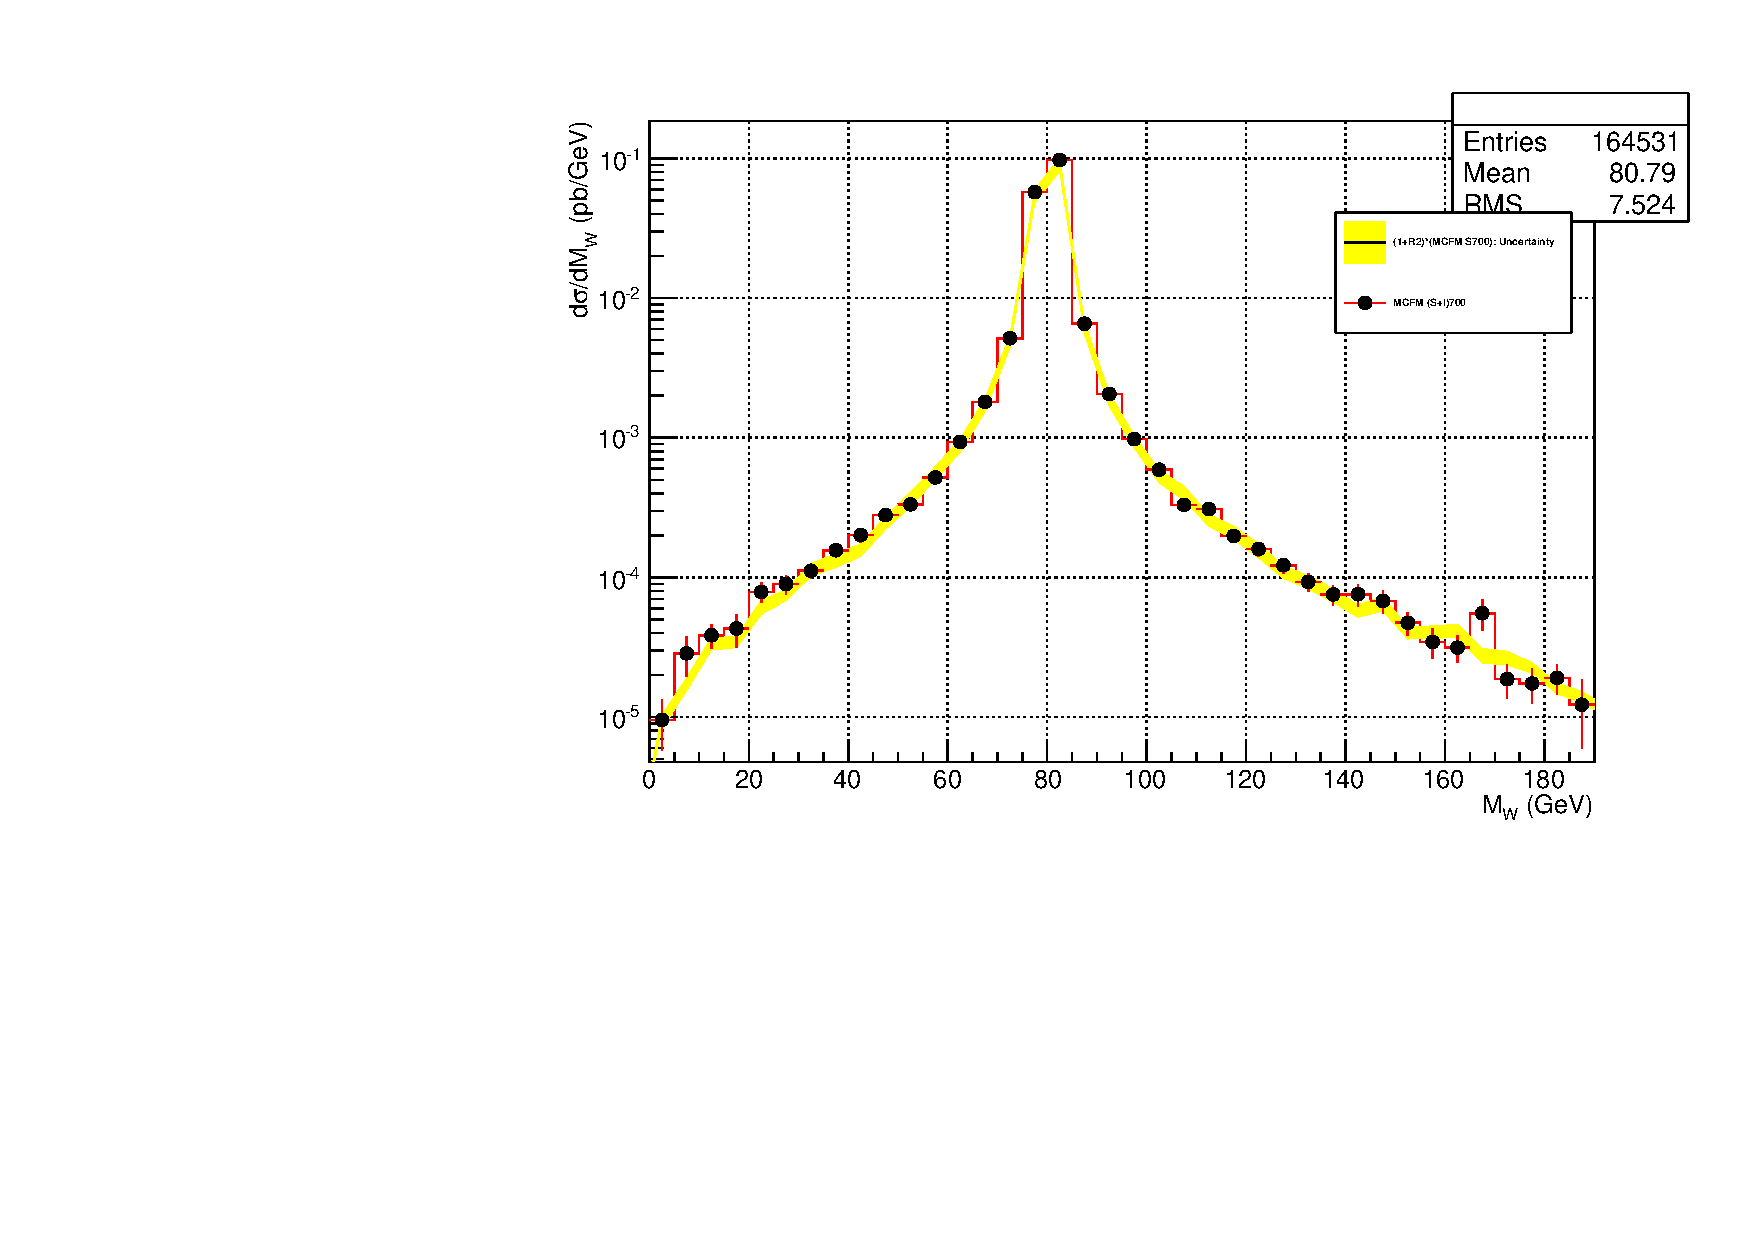
\includegraphics[width=0.42\textwidth]{plots/interference/mw.pdf}
    }
    \\
    \subfigure[$\eta_{l\nu}$]{
      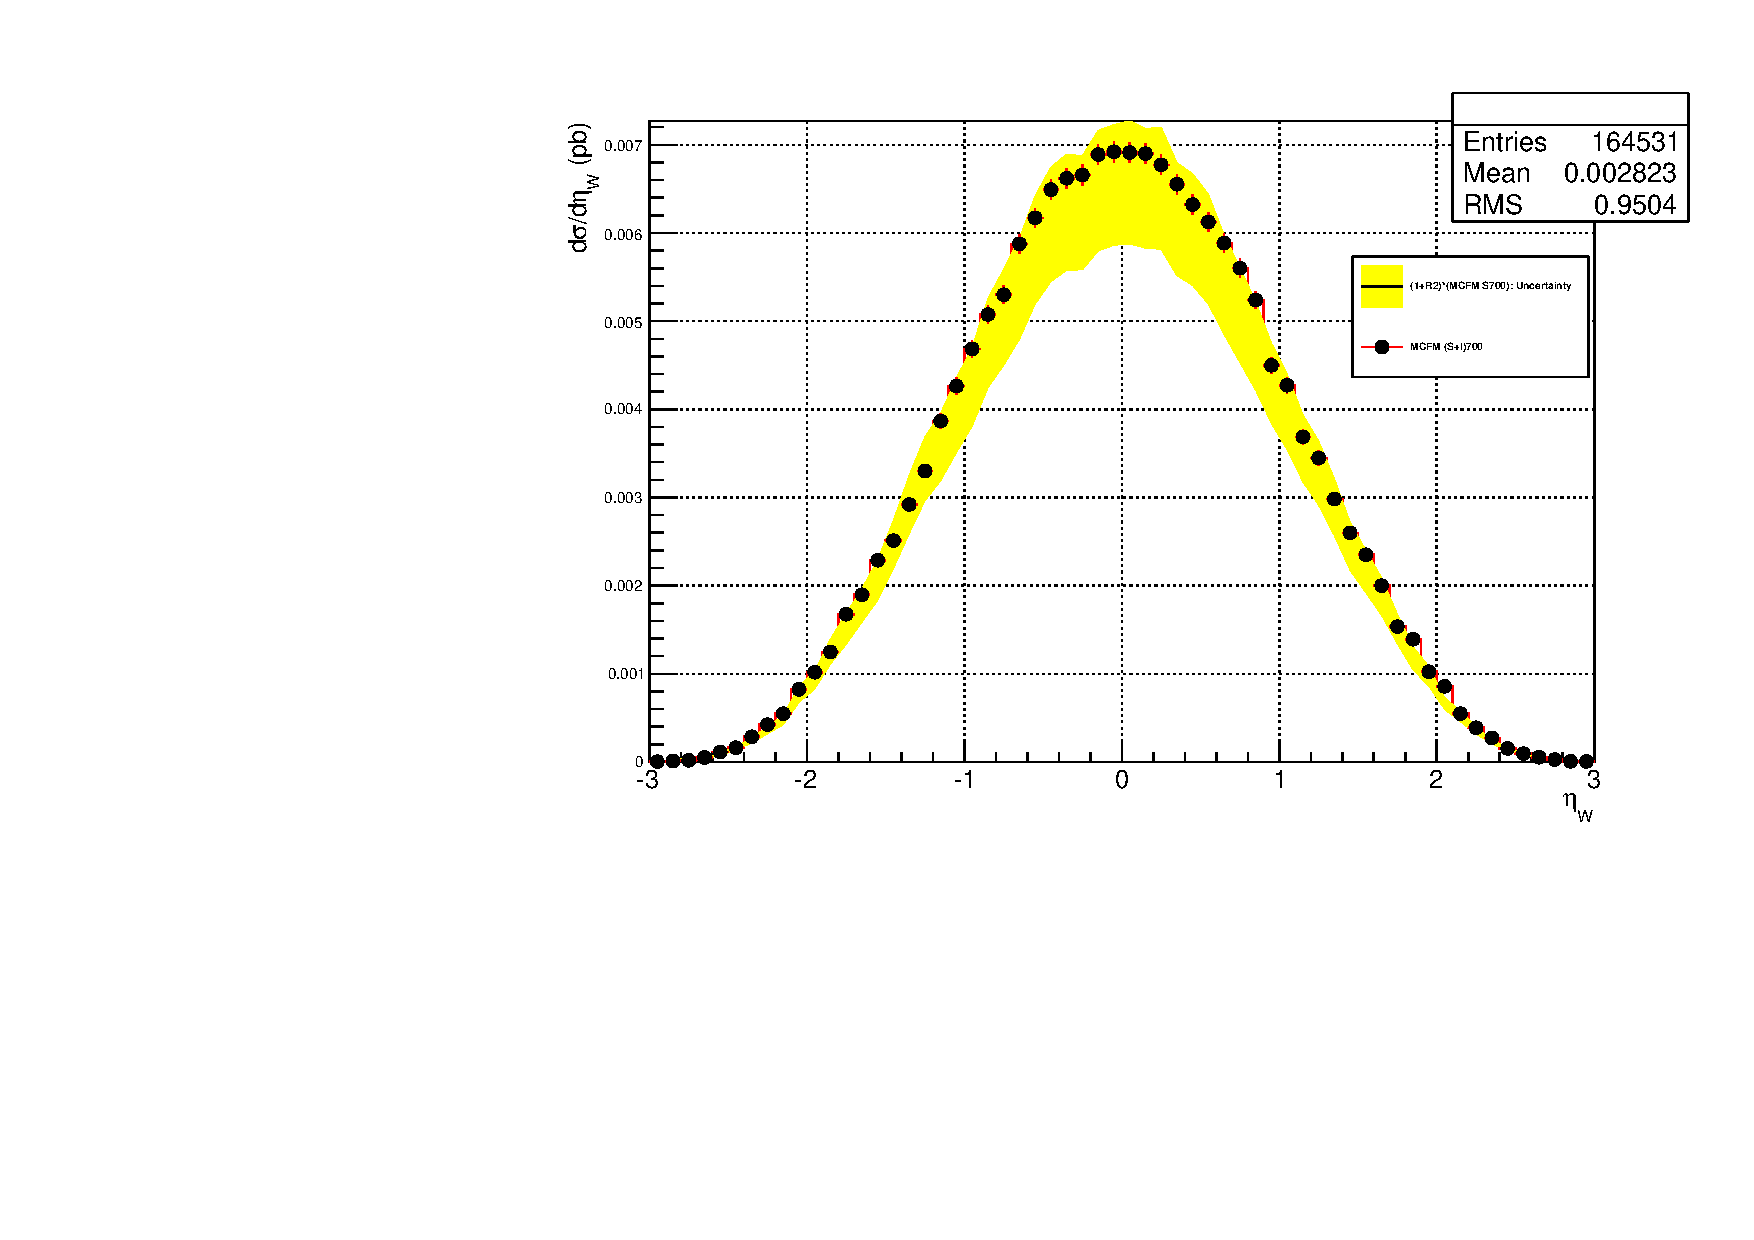
\includegraphics[width=0.42\textwidth]{plots/interference/etaw.pdf}
    }
    \subfigure[$P_{T,l}$]{
      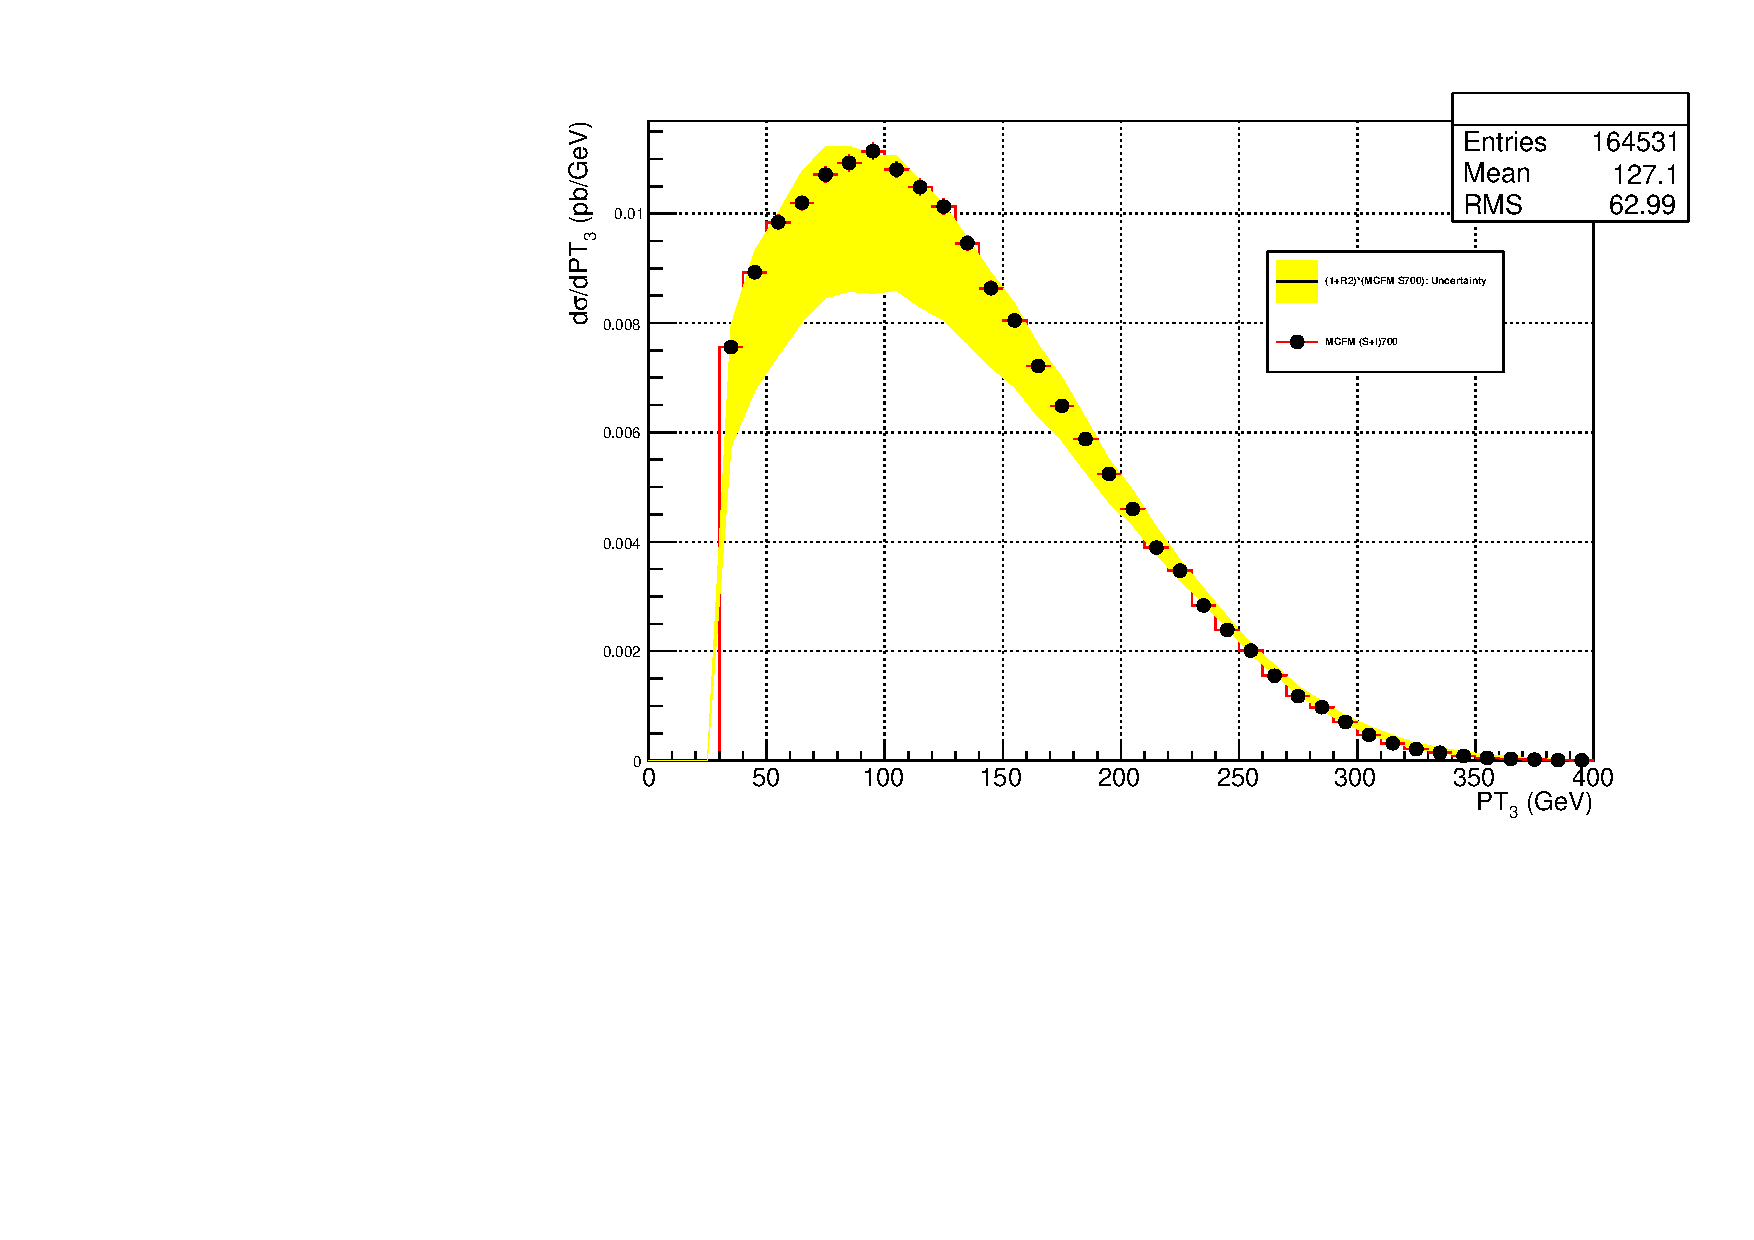
\includegraphics[width=0.42\textwidth]{plots/interference/pt3.pdf}
    }
    \\
    \subfigure[$\phi_{l,\nu}$]{
      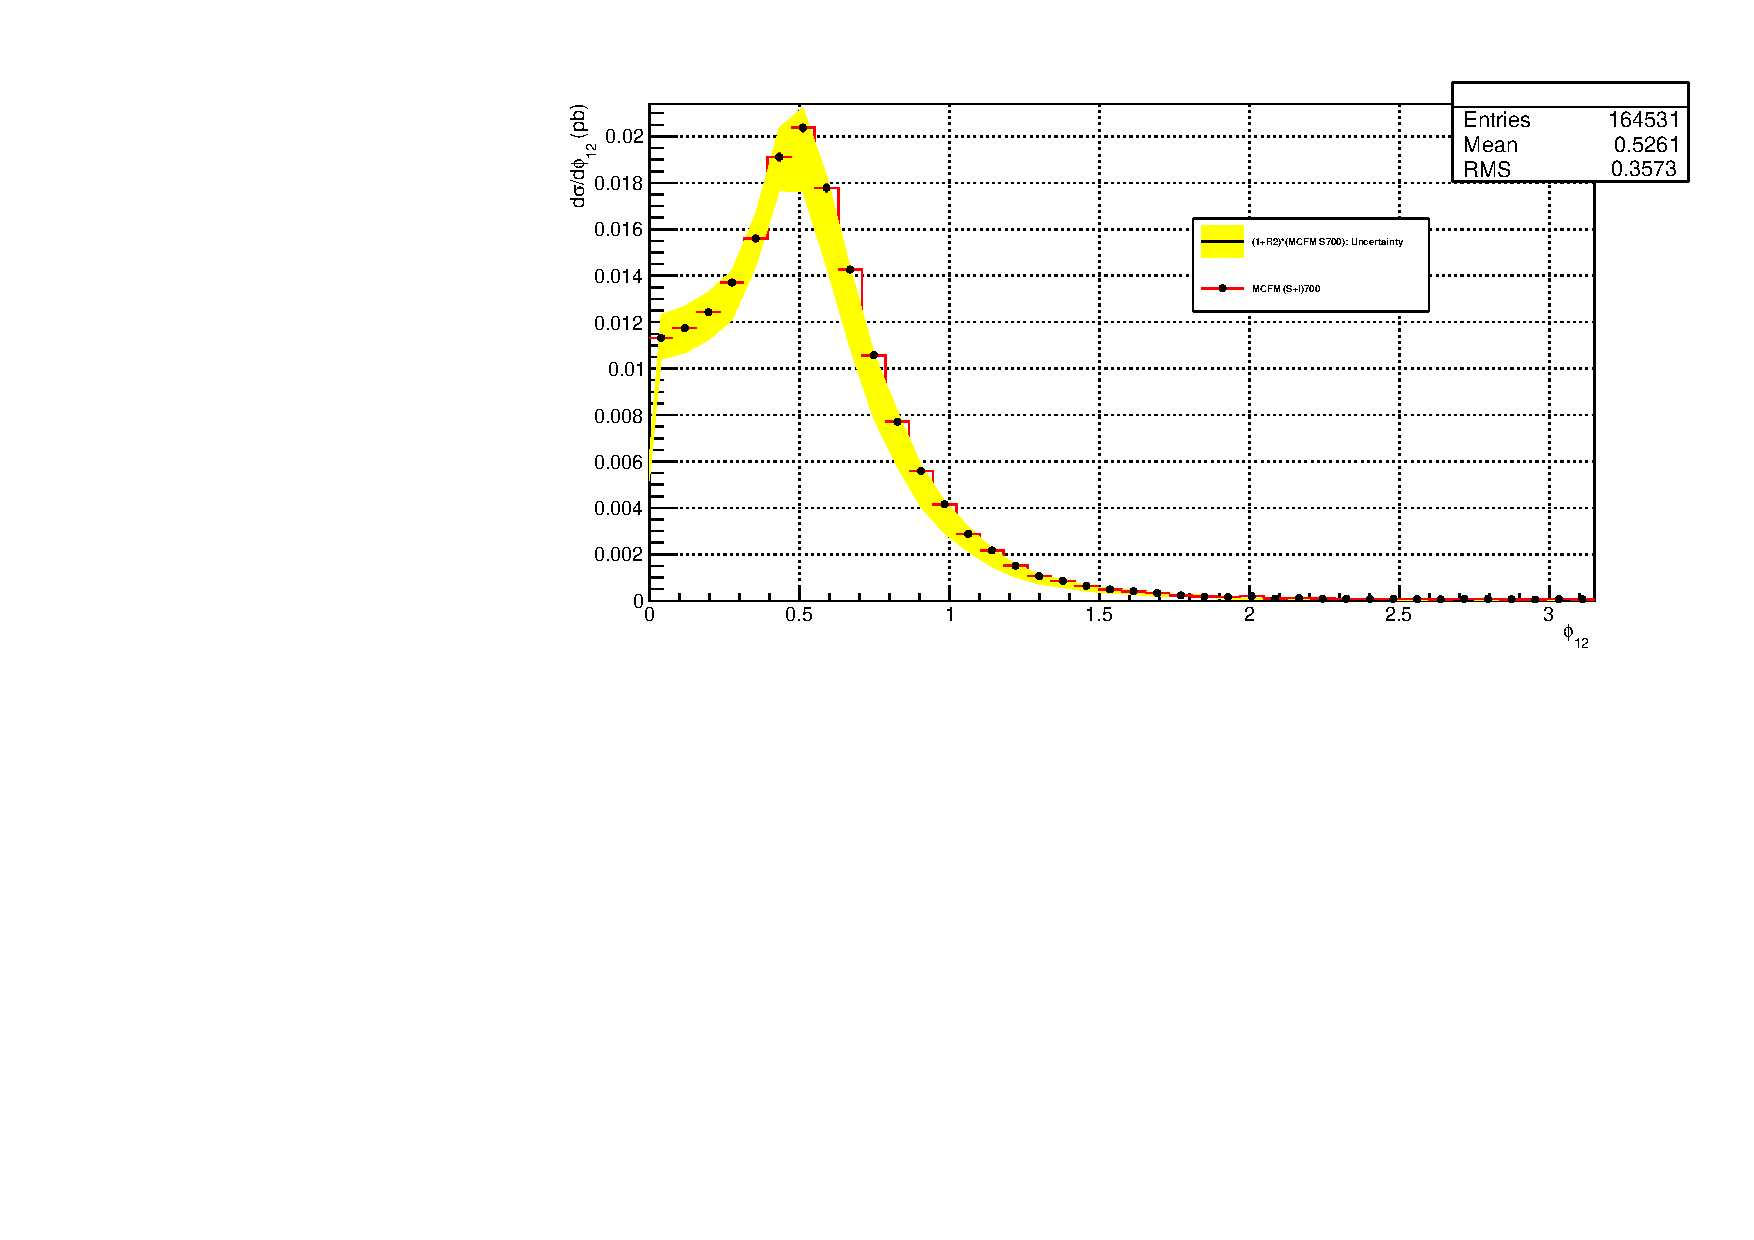
\includegraphics[width=0.42\textwidth]{plots/interference/phi12.pdf}
    }
    \subfigure[$\phi_{l,j}$]{
      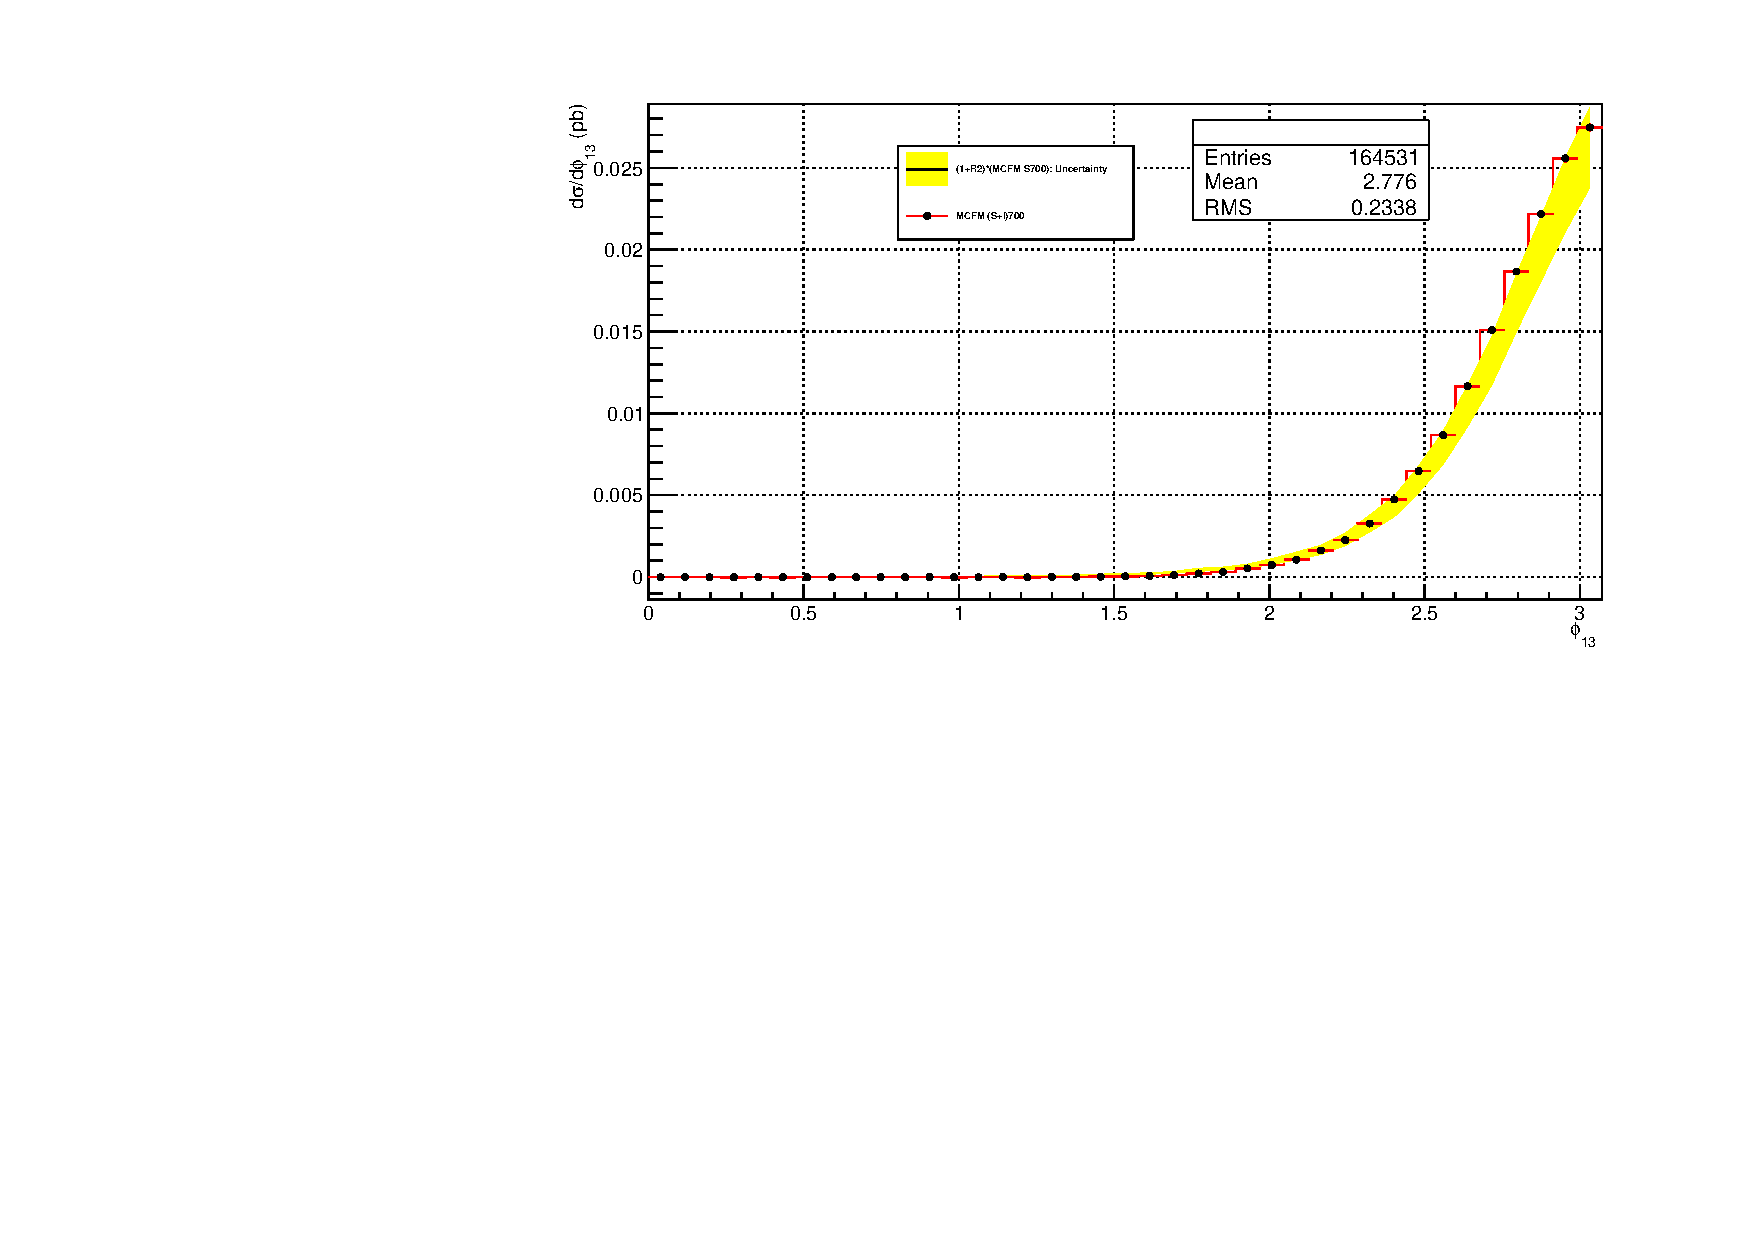
\includegraphics[width=0.42\textwidth]{plots/interference/phi13.pdf}
    }
    \caption{Reweighting MCFM $gg\to H \to WW \to l\nu jj$ with
    interference effects at the generator level, for $M_H=700$\,GeV at
    the 8TeV LHC, with $P_{T,l}>30$\,GeV, $P_{T,j}>30$\,GeV,
    MET$>30$\,GeV, and $|\eta_{l,j}|<2.4$. }
    \label{fig:MCFMHHIntfRew}
\end{figure}
%
